\documentclass{report}

\input{~/latex/template/preamble.tex}
\input{~/latex/template/macros.tex}

\title{\Huge{Declarations}}
\author{\huge{Matt Warner}}
\date{\huge{}}
\pagestyle{fancy}
\fancyhf{}
\rhead{}
\lhead{\leftmark}
\cfoot{\thepage}
% \usepackage[default]{sourcecodepro} \usepackage[T1]{fontenc}

\pgfpagesdeclarelayout{boxed}
{
  \edef\pgfpageoptionborder{0pt}
}
{
  \pgfpagesphysicalpageoptions
  {%
    logical pages=1,%
  }
  \pgfpageslogicalpageoptions{1}
  {
    border code=\pgfsetlinewidth{1.5pt}\pgfstroke,%
    border shrink=\pgfpageoptionborder,%
    resized width=.95\pgfphysicalwidth,%
    resized height=.95\pgfphysicalheight,%
    center=\pgfpoint{.5\pgfphysicalwidth}{.5\pgfphysicalheight}%
  }%
}

\pgfpagesuselayout{boxed}

\begin{document}
    \maketitle
\noindent Every object and function declaration has two main parts:
\begin{itemize}
    \item a sequence of one or more \textbf{declaration specifiers}.
    \item a \textbf{declarator} (or a seqence thereof, separated by commas).
\end{itemize}
\bigbreak \noindent
\begin{figure}[H]
\centering
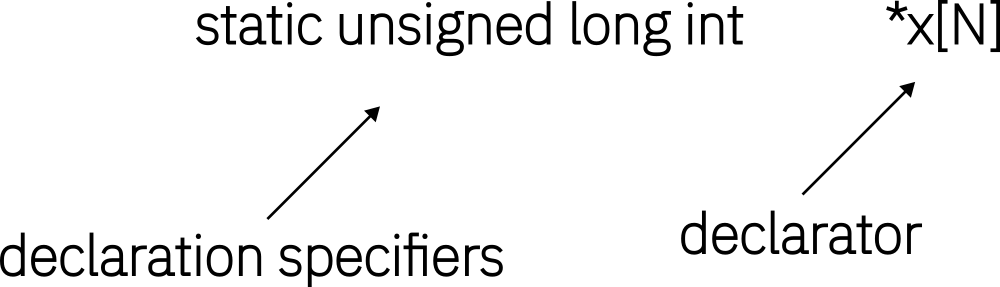
\includegraphics[width=0.35\textwidth]{ ./figures/1.png }
\caption{Structure of declarations}
\end{figure}
\noindent The \textbf{name declared} in a declarator is the \textit{\textbf{declarator-id}}. In the above example, the \textit{\textbf{declarator-id}} is $x$.
\bigbreak \noindent
Each \textbf{declaration specifier} is either:
\begin{itemize}
    \item a \textit{\textbf{type specifier}}
    \item a \textit{\textbf{non-type specifier}}
\end{itemize}
A type specifier can be:
\begin{itemize}
    \item A sequence of one or more keywords, such as \texttt{int}, \texttt{unsigned}, \texttt{long}, or \texttt{double}.
    \item An identifier or qualified name that names a type, such as \texttt{std:;string}.
    \item A template specialization, such as \texttt{vector<long double>}
\end{itemize}
A non-type specifer can be:
\begin{itemize}
    \item A \textit{\textbf{storage class specifier}}
        \begin{itemize}[label=$\circ$]
            \item A keyword such as \texttt{extern}, \texttt{static}, or \texttt{thread\_local}.
        \end{itemize}
    \item a \textit{\textbf{function specifier}}
        \begin{itemize}[label=$\circ$]
            \item A keyword such as \texttt{inline} or \texttt{virtual}.
        \end{itemize}
    \item Some \textit{\textbf{other specifier}}:
        \begin{itemize}[label=$\circ$]
            \item A keyword such as \texttt{friend} or \texttt{typedef}.
        \end{itemize}
\end{itemize}
A \textit{\textbf{declarator}} is a \textit{\textbf{declarator-id}} (the name being declared), possibly surrounded by operators.
\begin{itemize}
    \item unary * means ``pointer''
    \item unary \&& means ``lvalue reference''
    \item unary \&\& means ``rvalue reference''
    \item $[ \ ]$ means ``array''
        \item() means ``function''
\end{itemize}
\begin{figure}[ht]
\centering
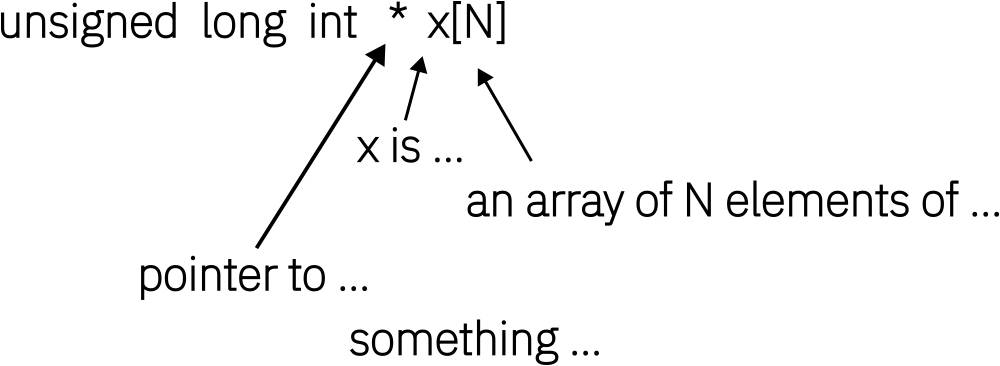
\includegraphics[width=0.42\textwidth]{ ./figures/2.png }
\end{figure}
In the above example, you would read that as ``x is an array of N elements of type pointer to unsigned long int"
\newpage
\noindent How do we know that \texttt{*x[N]} is an array of pointers and not a pointer to an array? The rule is fairly simple. The operators in a declarator group according to the same precedance as they do when they appear in an expression.
    \begin{figure}[H]
    \centering
     \setlength{\tabcolsep}{30}
    \begin{tabular}{ccc}
    \toprule 
    Precedence & Operator & Meaning \\
    \midrule
    Highest & ( ) & grouping \\
    \midrule
            & $[ \ ]$ & array \\
            & ( )  & function \\
            \midrule
    Lowest & \* & pointer \\
           & \& & reference \\
           & \&\& & rvalue reference \\
           \bottomrule


    \end{tabular}
    \end{figure}
\noindent    \texttt{*x[N]} is an array of pointers, because $[ \ ]$ has a higher precedence that unary *, so it takes effect first.
\bigbreak \noindent
Looking at the above table, you can see that parenthesis serve two roles in declarators:
\begin{itemize}
    \item As the \textit{\textbf{function call operator}}
        \begin{itemize}[label=$\circ$]
            \item These () follow the \textit{\textbf{delcarator-id}}
            \item They have the same precendence as $[ \ ]$
        \end{itemize}
    \item as \textit{\textbf{grouping}}
        \begin{itemize}[label=$\circ$]
            \item These () \textit{enclose} the declarator-id
            \item They have the highest precendence of all.
        \end{itemize}
\end{itemize}
\noindent For example:
\begin{minted}[linenos=false]{cpp}
void *f(int) // f is a function with parameter of type int returning void.

void (*f)(int) // f is a pointer to a function which takes an int and returns void.
\end{minted}
This is why when you write a function pointer you need those parenthesis enclosing the declarator. Otherwise,it means something different.
\end{document}

